\chapter{Forgiveness and Debts}
\vspace{0.6cm}
\begin{center}
\nopagebreak
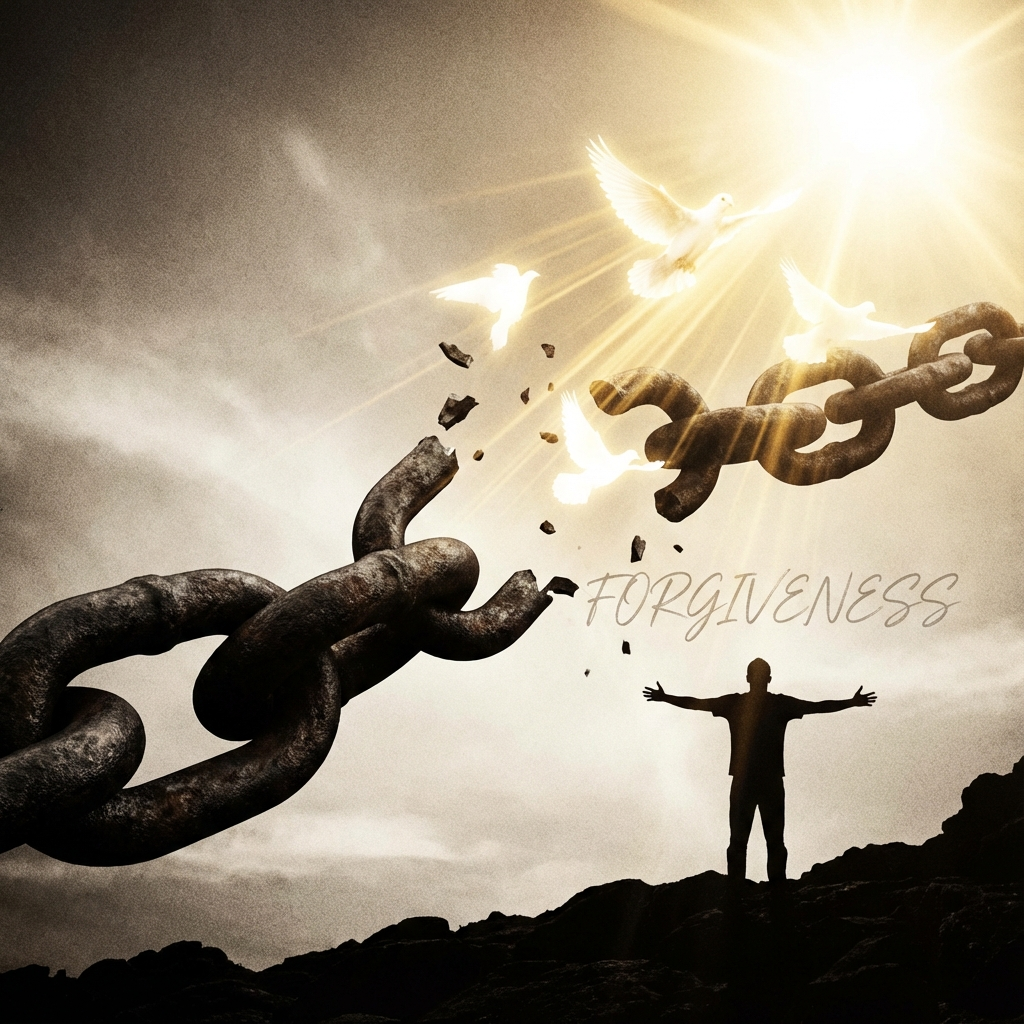
\includegraphics[width=0.75\textwidth,cfbox=gray!60 0.6pt 4pt]{forgiveness_chains.png}\\
\vspace{4pt}
{\small\itshape Conscious forgiveness: breaking quantum ties to the past.}
\end{center}

\vspace{0.6cm}
We returned to Las Rozas, to a quiet area. Jesus wanted to talk about something heavy.
—``Forgive us our debts, as we also forgive our debtors''.


—That's the difficult part —I admitted—. Forgiving someone who has hurt you...


—It's difficult because you see it as a favor you do for the other person. ``I, who am so good, forgive you, who are so bad''. That is ego. That is useless.


—Then?


—Forgiveness is an act of personal hygiene. It is letting go of a burning coal that you were holding, waiting to throw it at someone else. The only one who gets burned is you.


He sat on a stone bench.
—When you hold a grudge, you vibrate very low. You tie yourself to that person and to that painful moment with an invisible chain. You can't fly. You can't move forward. Forgiving is cutting the chain. It is saying: ``I release you and I release myself. I no longer owe you anything, and you owe me nothing''.


—And if what they did was very serious?


—Pain is inevitable, suffering is optional. If you keep reviewing the offense in your mind, you are reliving it over and over again. You are hurting yourself now, not the other person. ``Deliver us from evil'' starts by delivering yourself from the evil you yourself generate by not forgiving.


He put his hand on my shoulder.
—Forgiving is vibrating so high that the offense no longer reaches you. It is understanding that the other person acted from their own unconsciousness, from their own pain. ``They know not what they do''. If they knew the damage they do to themselves by damaging another, they would not do it.